\chapter{Notations and Abbreviations}
\section{Common Acronyms and Notations}\label{s:app}
\begin{itemize}
\item LS: least square.
\item WLS: weighted least square.
% \item OED: optimal experiment design.
\item FIM: Fisher information matrix.
\item CRLB: Cram\'{e}r-Rao lower bound.
\item WSN: wireless sensor network.
\item TDOA: time difference of arrival.
\item TOA: time of arrival.
\item TOF: time of flight.
\item POA: phase of arrival.
\item Vectors and matrices: vectors are typed in bold math font, such as vector $\mathbf{v}$. Matrices are indicated by capital math font, e.g., $M$. Note that random variable is denoted by bold capital font, e.g., $\mathbf{X}$. Thus, $\mathbf{p} \neq p \neq P \neq \mathbf{p}$, since $\mathbf{p}$ is a vector, $p$ is a scalar, and $P$ is a matrix. By default, all vectors are column vectors. For example, $\mathbf{p}=\left(
                        \begin{array}{c}
                          p_1 \\
                          p_2 \\
                          \vdots \\
                          p_n \\
                        \end{array}
                      \right) = \left(
                        \begin{array}{c}
                          \mathbf{p}_{(1)} \\
                          \mathbf{p}_{(2)} \\
                          \vdots \\
                          \mathbf{p}_{(n)} \\
                        \end{array}
                      \right).$
 Note that $\mathbf{p}_{(1)}$ is the first entry of the vector $\mathbf{p}$, and $\mathbf{p}_{(1)}$ is a scalar. $\mathbf{p}_1$ is a vector. By default, $M$ and $M_1$ are two difference matrices, and $M\neq M_1$.
\item Subscripts: the subscripts in brackets indicate scalar entries of a matrix or vector. The subscripts without brackets are instances of variables. Capital subscripts are parts of the variable's name. So, $t$ and $t_A$ are different scalars. Lower case subscripts, e.g., $i,j,k$, are used as indices for positive integers. For example, $\mathbf{p}_{(i)}$ is the $i$th entry of the vector $\mathbf{p}$, and $\mathbf{p}_{(i)}$ is a scalar.
  Similarly, $M_{(i,j)}$ is the $i$th row and $j$th column scalar entry of matrix $M$. $M_{(i,:)}$ is the $i$th row vector of matrix $M$, and $M_{(:,i)}$ is the $i$th column vector of matrix $M$.
    $\mathbf{p}_i$ is the $i$th $\mathbf{p}$ vector, where $i=1,2,3,\cdots$. Note that $p_i$ is the $i$th $p$, and $p_i$ is a scalar. Thus, $\mathbf{p}_i\neq p_i$.  However, $\mathbf{p}_{(i)}=p_i$ by default, and both of them are scalars. % Finally, this is a complex example: $M_{Ai(2,:)}^T$.
\end{itemize}

\section{Notations in {Chapter~\ref{s:MasnetIROS}}}
%\section{Notations in Chapter 2}
\begin{itemize}
\item $m$: the weight of one robot.
\item $I$: the inertia of the robot along the $z$ axis. Note that $I$ is a scalar. In the literature, $\mathcal{M}$ can be a 3 by 3 inertia matrix of the robot. The $I$ in (\ref{e:ddmodel}) is the entry at the 3rd row and 3rd column of $\mathcal{M}$, i.e. $\mathcal{M}_{(3,3)}$.
\item $l$: the length of the robot's axis.
\item $r$: wheel radius. The left and right wheels have the same radius.
\item $\alpha$: the yaw angle as shown in Fig.~\ref{fig:ddrive}.
\item $(x,y)$: the coordinate of the center of the axis. Note that $\mathbf{x}$ is not $x$.
\item $\tau_l$,$\tau_r$: the torque applied on the left and right wheel, respectively. $\tau=[\tau_l \tau_r]^T$.
\item $A$, $B$, $\mathbf{x}$, $\tau$: the parameters, states, and the control signal for a single robot.
\item $A_T$, $B_T$, $\mathbf{x}_T$, $\tau_T$: the parameters, states, and the control signal for three robots.
\item $b$: the edge length of the robot's square chassis. It is assumed that the wheels and the axis are mounted on a square chassis.
\item $\chi(t)$: Mayer state.
\item $\chi_{dl}(t)$: stacks all the entries on the diagonal and below the diagonal of $\chi$ to a vector.
\item $\Omega$: the domain for valid input variables.
\item $\partial\Omega$: the boundary of $\Omega$.
\item $n$: number of robots.
\item $\mathbf{c}$: the vector of unknown parameters. $\mathbf{c}=[c_1, c_2, c_3]^T$.
\end{itemize}

\section{Notations in Chapter~\ref{s:COSS}}
%\section{Notations in Chapter 3}
\begin{itemize}
\item $n$ : the total number of sensors. Note that $n\neq \mathbf{n}$.
\item $n_i$, or $\mathbf{n}_{(i)}$: the number of samples that sensor $i$ collects in each $t_S$, the sampling period. Note that $\mathbf{n}=[n_1, n_2,\cdots]^T\neq n$. %when $i\neq0$, $n_i$ is the number of samples that sensor $i$ collects in $T_{t}$. At the initial stage, each sensor collect the same number of samples and send the average of the samples to sink. The initial number of samples is $n_0$. $n_0=c_t/N$.
\item $P_r$: probability function.
\item $m$: the number of parameter for identification.
\item $t_S$: the total sampling time. In $t_S$, sensor $i$ collects
$n_i$ samples.
\item $n_{S}$: the max total number of samples of the whole WSN in $t_S$ time slot.
\item $c_{1}$, $c_2$, etc: the coefficients in sensor model.
\item $\sigma_{i}$, $\bar{\sigma}_{i}$, $\tilde{\sigma}_i$: $\sigma_{i}$ is the standard deviation of the noise of the $i$th sensor. $\bar{\sigma}_{i}$ is the standard deviation for the $i$th averaged sensor measurement. $\tilde{\sigma}_i$ is similar to $\bar{\sigma}_{i}$ but averaged over nominal sampling rates.
%\item $f(k)$: the value of function $f$ at the time instance $k$.
\item $f[k]$: the value of function $f$ for the $k$-th iteration.
\item $y_i$ or $\mathbf{y}_{(i)}$: the nominal value of sensor $i$. It is computed by the model of events.
\item $v_{i}$: the noise of sensor $i$.
\item $s_i$ or $\mathbf{s}_{(i)}$: real value of the reading of sensor $i$. $s_{i}[k]:=y_{i}[k]+v_{i}[k]$.
\item $\bar{s}_{i}$: averaged sensor $i$'s reading.
\item $\mathcal{N}(\mu,\sigma)$: Gaussian (normal) distribution with the
expectation of $\mu$ and variance of $\sigma$.
\item $\mathbf{p}$: normalized sampling rate of sensor $i$. %As a variation,
$\hat{\mathbf{p}}[k]$ is the optimized normalized sampling rate for the $k$-th iteration.
\item $\mathbf{r}_{i}$: position of sensor $i$. $\mathbf{r}_{i}$ is assumed
precisely known. In addition $\mathbf{r}_{i}\neq\mathbf{r}_{j}$,
for any $i\neq j$. By default, $\mathbf{r}_{i}$ is a 2D vector like
$\left(\begin{array}{c}
x_{i}\\
y_{i}\end{array}\right)$. % with $\mathbf{r}_{i(x)}=x_i$ and $\mathbf{r}_{i(y)}=y_i$.
\item $\mathbf{q}$, $\mathbf{q}^\ast$: $\mathbf{q}$ is the nominal position of the target. Specifically, $\mathbf{q}^\ast$ is the true position of the target.
\item $\mathbf{1}$: an all-one vector, i.e., $[1, 1, \cdots, 1]^T$.
\item $\nabla$: gradient. For example, $\nabla_{\mathbf{q}}$ is the gradient
with respect to $\mathbf{q}$.
\item $\mathbf{a}\geq b$: each entry of vector $\mathbf{a}$ is no less than the scalar $b$. $a_{i}\geq b$. E.g., $\mathbf{p}\geq 0$.
\item $A\succeq B$: matrix $A-B$ is positive semi-definite.
\end{itemize}

\section{Notations in Chapter~\ref{s:loc}}
%\section{Notations in Chapter 4}
\begin{itemize}
\item $\Omega$: the domain for deploy mobile node and beacons.
\item $\mathbf{q}_i$: the position of the $i$th beacon.
\item $\mathbf{p}_i$: the position of the $i$th mobile node.
\item $m$: number of mobile nodes.
\item $n$: number of beacons.
\end{itemize}

\chapter{Fisher Information for Error Bound Estimation}~\label{s:fi}
Fisher information is a metric to indicate the sensitivity of the measurements with respect to system parameters. The definition of Fisher information and Fisher information matrix is presented by Definition~\ref{d:fisher} in Section~\ref{s:MasnetIROS}.
%\begin{mdef}\label{d:fisher}
%If a measurable random variable $X$ depends on parameter $\theta$, and the likelihood function is $l(\theta;X)$.
%Then the Fisher information is
%\begin{equation*}
%    \mathcal{I}=E\{[\frac{\partial}{\partial \theta} \log l(\theta;X)]^2 \}
%\end{equation*}
%The matrix form is Fisher information matrix, which is $M$, with the $i,j$th entry defined as:
%\begin{equation*}
%    M_{(i,j)}=E\{\frac{\partial}{\partial \theta_i} \log l(\theta;X) \frac{\partial}{\partial \theta_j} \log l(\theta;X) \}
%\end{equation*}
%\end{mdef}

Following the convention in Definition~\ref{d:fisher}, let $P_r(X)$ be the probability density function of the random variable $X$.
Easy to see, if $P_r(X;\theta)$ is independent Gaussian, the sensitivity for each sensor can be computed separately.
% Eq.~\ref{e:m} is the Fisher information matrix.
\begin{eqnarray*}
% \nonumber to remove numbering (before each equation)
  l(\theta;X) &=& \frac{1}{\sqrt{2\pi}\sigma} \exp(-\frac{(X(\theta)-\mu)^2}{2\sigma^2})\\
  M_{(i,j)} &=& E\{\frac{\partial}{\partial \theta_i} \log l(\theta;X) \frac{\partial}{\partial \theta_j} \log l(\theta;X) \} \\
%  M_{(i,j)}&=& E\{\frac{\partial}{\partial \theta_i}(-\ln(\sqrt{2\pi\sigma^2})-\frac{(X(\theta)-\mu)^2}{2\sigma^2})
%    \frac{\partial}{\partial \theta_j}(-\ln(\sqrt{2\pi\sigma^2})-\frac{(X(\theta)-\mu)^2}{2\sigma^2}) \}\\
  M_{(i,j)} &=& E\{\frac{(X-\mu)^2}{\sigma^4}\frac{\partial X}{\partial \theta_i}\frac{\partial X}{\partial \theta_j} \} \\
  M_{(i,j)} &=& \frac{1}{\sigma^2} \frac{\partial X}{\partial \theta_i}\frac{\partial X}{\partial \theta_j}
\end{eqnarray*}
Thus, (\ref{e:mTraj}), (\ref{e:mSSP}) and (\ref{e:bplocFIM}) are the Fisher information matrices.

%A related concept is Fisher information entropy. Paper~\cite{RomeraFisherEntropy99} formulates Fisher information entropy for a 3D particle system as $\mathcal{I}_f$,
%\begin{equation}\label{e:fentropy}
% \mathcal{I}_f = \int [\|\nabla f(\mathbf{r})\|^2 /f(\mathbf{r}) ] \hbox{d}\mathbf{r},
%\end{equation}
%where $f(\mathbf{r})=f(x,y,z)$ is the pdf for a particle appears at the position $\mathbf{r}$.


\begin{thm}[Cram\'{e}r-Rao inequality \cite{MoonSig} p.551]
If $t(\theta)$ is any unbiased estimator of $\theta$ based on a differentiable likelihood function, then
\begin{equation} \label{e:crlb}
    E\{(t(\theta)-\theta) (t(\theta)-\theta)^T\} \geq M^{-1}(\theta),
\end{equation}
where $M(\theta)$ is the Fisher information matrix (FIM).
\end{thm}
\begin{remark}
According to this theorem, the inverse of the FIM is the indicator for the minimum possible covariance of any unbiased estimators. In fact, if the maximum likelihood estimator, $\theta_{ML}$, exists, the following equation holds~\cite{EmeryOED98}:
$$E\{(\theta_{ML}-\theta)(\theta_{ML}-\theta)^T\}=M^{-1}(\theta). $$
In other words, reducing the right hand side of (\ref{e:crlb}) actually improves the estimator $\theta_{ML}$, if it exists.
%if we can find an unbiased estimator $\bar{t}(\theta)$ achieve the CRLB, or $ E\{(\bar{t}(\theta)-\theta) (\bar{t}(\theta)-\theta)^T\} = M^{-1}(\theta)$, then $\bar{t}(\theta)$ is called efficient.
%    Although it is possible that a biased estimator has less error
%If we have a
\end{remark}


%\chapter{Mathematical Background}
%\section{Derivatives of Matrices}
%\section{Linear Programming}
%\section{Convex Constraint Optimization}

\chapter{Implementations}
\section{Simulation on Trajectory Optimization}
This section presents the implementation on simulations in Chapter~\ref{s:MasnetIROS}. Table~\ref{t:egRiots} is an example of how to set up common parameters of the simulation and how to invoke the \texttt{riots} function.  Tables~\ref{t:egSysInit}, \ref{t:egSysH} and \ref{t:egSysG} are the examples of two key functions for the \texttt{riots} function. \verb!sys_init.m! is the initialization function for the optimization. The robots' dynamics model is formulated in \verb!sys_h.m!, while the optimization criteria is presented in \verb!sys_g.m!. The variable \verb!Sensitivity! the sensitivities on some points, and it is  computed by the Matlab PDE toolbox. The function \verb!Interpolate! is a function to interpolate sensitivity values.

%\subsection{Parameters}
\lstset{language=Matlab, breaklines=true, numbers=left, texcl, mathescape=true }


\begin{table}[!h]
  \centering
  \caption{An Exemplary Setting for RIOTS Simulations}\label{t:egRiots}
\begin{lstlisting}
m=0.05; % weight of each robot: 0.05 kg
b=0.08; % edge length of each robot: 8 cm
l=0.08; % length between the two wheels of a robot: 8 cm
I=m*b*b*2/12; % inertial of a robot with respect to the z-axis
r=0.04; % radius of the wheel: 4 cm
MinU = -100; % bound of the input torque is positive and negative 100 kg-m
MaxU =  100;
s0 = [0.2; 0.1; 15/180*pi; zeros(3,1);... % The initial states of the 1st robot: initial position is (0.2, 0.1). Initial orientation is 15 degree and the initial linear and rotatory speeds are all 0.
      0.2; 0.5; 15/180*pi; zeros(3,1); ... % The initial states of the 2nd robot
      0.2; 0.8; 15/180*pi; zeros(3,1)]; % The initial states of the 3rd robot
BoundXY=1; %
BoundVelocity=0.5; % 0.5 m/s
BoundAlpha=2; % 2 rad/s
NumberOfParameters=3; % to observe three parameters: C1, C2, C3
NumberOfMayerVariable = NumberOfParameters*(NumberOfParameters+1)/2; % compute to number of Mayer states as the augmentation of robot's state variables.
x0 = [s0; zeros(NumberOfMayerVariable, 1)];
NumberOfSensorStates=6*3; % there are three robots with 6 internal states for each one.
fixed = [ones(NumberOfSensorStates, 1); zeros(NumberOfMayerVariable, 1)]; % Inform riots which variables are fixed thus should not be optimized by assigning 1 to the associated values in the ``fixed" vector.
X0 = [x0, fixed, x0_lower, x0_upper];
[u_optml, x_optml, f] = riots(X0, u0, TGRID, -u_max*ones(n_ctrls,1), u_max*ones(n_ctrls,1),[], [80, 0, 1], 4);
\end{lstlisting}
\end{table}


\begin{table}[htb]
  \centering
  \caption{An Example of the \texttt{sys\protect\underline{\ }init.m} File for RIOTS} \label{t:egSysInit}
\lstset{language=Matlab, breaklines=true, numbers=left, texcl=false, mathescape=true}
\begin{lstlisting}
function neq = sys_init(params)
global Sensitivity NumberSensors
StatesPerSensor=6; % for differentially-driven robots
if isempty(params)
    NumberControls = 2 * NumberSensors;
    NumberParameters = size(Sensitivity, 4);
    NumberStates = StatesPerSensor * NumberSensors + NumberParameters * (NumberParameters + 1) / 2;
    %    6 states for each differential drive robot
    %    n*(n+1)/2 is the number of unique entries in the FIM
    neq = [1 NumberStates; 2 NumberControls ];
    % neq = 1  : number of state variables.
    % neq = 2  : number of inputs
else
    global SysParams
    SysParams = params;
end
return
\end{lstlisting}
\end{table}


\begin{table}[htb]
  \centering
  \caption{An Example of the \texttt{sys\protect\underline{\ }h.m} File for RIOTS}\label{t:egSysH}
  \lstset{language=Matlab, breaklines=true, numbers=left, texcl, mathescape=true }
\begin{lstlisting}
function xdot = sys_h(neq, t, x, u)
global SysParams IndexMayerVariable NumberSensors
global b m l I r
% xdot must be a column vector with n rows.
StatesPerSensor=6; % for differentially-driven robots
NumberSensorDynamics = NumberSensors * StatesPerSensor;
NumberParameters=round(sqrt(IndexMayerVariable(end)));
x1 = x(1: StatesPerSensor: NumberSensorDynamics - 1); % x1 is the x-axis
x2 = x(2: StatesPerSensor: NumberSensorDynamics); % x2 is the y-axis
% the states of one robot is x=[x1 x2 alpha dx1 dx2 dalpha]'
g = InterpolateSensitivities(x1, x2, t, neq(4));
a = zeros(NumberParameters, NumberParameters);
for loop = 1: NumberSensors
    a = a + g(loop, :)' * g(loop, :);
end
A33=[-2*b/m 0 0 ; 0 -2*b/m 0; 0 0 -b*l*l/(2*I)];
A1=[zeros(3) eye(3); zeros(3) A33]; % the A matrix for one robot
A=[A1  zeros(size(A1,1), size(A1,2)*(NumberSensors-1) )];
for cnt=1:NumberSensors-1
    A=[A; zeros(size(A1,1), size(A1,2)*cnt)  A1  zeros(size(A1,1), size(A1,2)*(NumberSensors-1-cnt)) ];
end
% A is comparable to A1, but for n sensors
NumberPhysicalState=NumberSensors*StatesPerSensor;
B=[];
Zero=zeros(StatesPerSensor, 2);
alpArray=x(3:StatesPerSensor:NumberPhysicalState);
for cnt=1:NumberSensors
    alp=alpArray(cnt);
    B1=[zeros(3,2);...
            r*cos(alp)/m r*cos(alp)/m;...
            r*sin(alp)/m r*sin(alp)/m;...
            -r*l/(2*I)   r*l/(2*I)];
    B=[B; repmat(Zero, 1, cnt-1) B1  repmat(Zero,1, (NumberSensors-cnt))];
end
xdot = [A*x(1:NumberPhysicalState)+B*u; a(MayerVariable)];
return
\end{lstlisting}
\end{table}


\begin{table}[htb]
  \centering
  \caption{An Example of the \texttt{sys\protect\underline{\ }g.m} File for RIOTS}\label{t:egSysG}
\lstset{language=Matlab, breaklines=true, numbers=left, texcl, mathescape=true }
\begin{lstlisting}
function J = sys_g(neq, t, x0, xf)
global SysParams IndexMayerVariable

StatesPerSensor=6;
NumberSensors = round(neq(2) / 2);
NumberPhysicalState=NumberSensors*StatesPerSensor;
NumberParameters=round(sqrt(IndexMayerVariable(end)));
NumberSensorDynamics = neq(1);
FNum = neq(5);
if FNum == 1
    fim = zeros(NumberParameters, NumberParameters);
    fim(IndexMayerVariable) = xf(NumberPhysicalState+1: end); % comput FIM based on the Mayer states
    fim = fim';
    fim(IndexMayerVariable) = xf(NumberPhysicalState+1: end);
    J = -log(det(fim));
else
    error('Reference to a non-existing constraint on initial/final state')
end
return
\end{lstlisting}
\end{table}


\clearpage
\section{Sensor Selection Demo System}
\subsection{Exemplary Matlab Code}
The exemplary sensor selection code is shown in Table~\ref{t:egCOSScode}, with the following comments on the variables.

\begin{itemize}
\item \texttt{NSample}: the total number of samples.
\item \texttt{SenPos}: positions of all the sensors.
\item \texttt{C},\texttt{LampHeight}: parameters of the lamp.
\item \texttt{sigma}: standard deviation.
\item \texttt{eta}: tuning knob of the sampling rate optimization.
\end{itemize}

\begin{table}
\caption{Exemplary Sensor Selection Code}\label{t:egCOSScode}
%\small
%\renewcommand{baselinestresh}{0.5}
\begin{lstlisting}[language=Matlab]
SenVal=SensorDataWithNoise(SelSenPos, LampPos); % collect sensor data
Pos0=mean(SenPos,2);
LSDat=struct('SenPos',SenPos,'SenVal',SenVal,'C',C,'LampHeight',LampHeight);
Optset=optimset('fmincon');
Pos1=fmincon(@EnergyErr, Pos0, [],[],[],[], ...
    [0;0], [GridNumX; GridNumY]*GridSizeIn*in2cm, [], Optset, LSDat);
SenST = SensitivityComp(SenPos, Pos1, 'energy');
ErrM1=zeros(2,2);
for cnt=1:SensorNum;
    ErrM1=ErrM1+sigma^(-2)*SenST(:,cnt)*SenST(:,cnt)' ... *round(NSample/SensorNum);
    end
plotEllipse(Pos1,inv(ErrM1),':k');
p=SampOpt(Pos1, SenST, sigma, eta);     % Sampling rate optimization
SenInd = find(p>=ThresholdSelection);
SelSenP = p(SenInd);
SelSenPos=SenPos(:,SenInd);
SelSenVal= SensorDataWithNoise(SelSenPos, LampPos); % collect another set of sensor data
LSDat2=struct('SenPos',SelSenPos,'SenVal',SelSenVal,'C',C,'LampHeight',LampHeight);
Pos2=fmincon(@EnergyErr, LampPos, [],[],[],[], ...
    [0;0], [GridNumX; GridNumY]*GridSizeIn*in2cm, [], Optset, LSDat2);
SenST2 = SensitivityComp(SelSenPos, Pos2, 'energy');
ErrM2=zeros(2,2);
for cnt=1:size(SenST2,2);
    ErrM2=ErrM2+sigma^(-2)*SenST2(:,cnt)*SenST2(:,cnt)' * round(NSample*SelSenP(cnt));
end
h2ball=plotEllipse(Pos2,inv(ErrM2),'g');
h2pos=plot(Pos2(1),Pos2(2),'xg');
h2SelSen=plot(SelSenPos(1,:),SelSenPos(2,:),'rs');
return
\end{lstlisting}
\end{table}


\begin{table}
\caption{Exemplary Code for Sensitivity Computation}\label{t:senst}
\begin{lstlisting}
function SenST=SensitivityComp(Pos, LampPos)
% Pos: the position of each sensor node
% LampPos: the position on the lamp
global C
SenN=size(Pos,2);
SenVal = SensorModel(Pos, LampPos); % nominal value, without error
Len=size(Pos,2);
SenST=zeros(2,Len);
for cnt=1:Len
    SenST(:,cnt) = 2*(Pos(:,cnt)-LampPos)*(SenVal(cnt).^2)'/C;
end
return
\end{lstlisting}
\end{table}



%\begin{table}
%\caption{}
%\begin{lstlisting}
%function h=plotEllipse(center,M,str)
%w=linspace(0,2*pi);
%unitV=[cos(w); sin(w)];
%pt=[];
%for cnt=1:length(w);
%    pt=[pt center + M*unitV(:,cnt)];
%end
%h=plot(pt(1,:), pt(2,:), str);
%\end{lstlisting}
%\end{table}
%\subsection{Exceptional Handling in C\#}

\subsection{Experimental Data}
The following data are collected during the experiments on our sensor selection testbed.

\begin{figure}
\centering
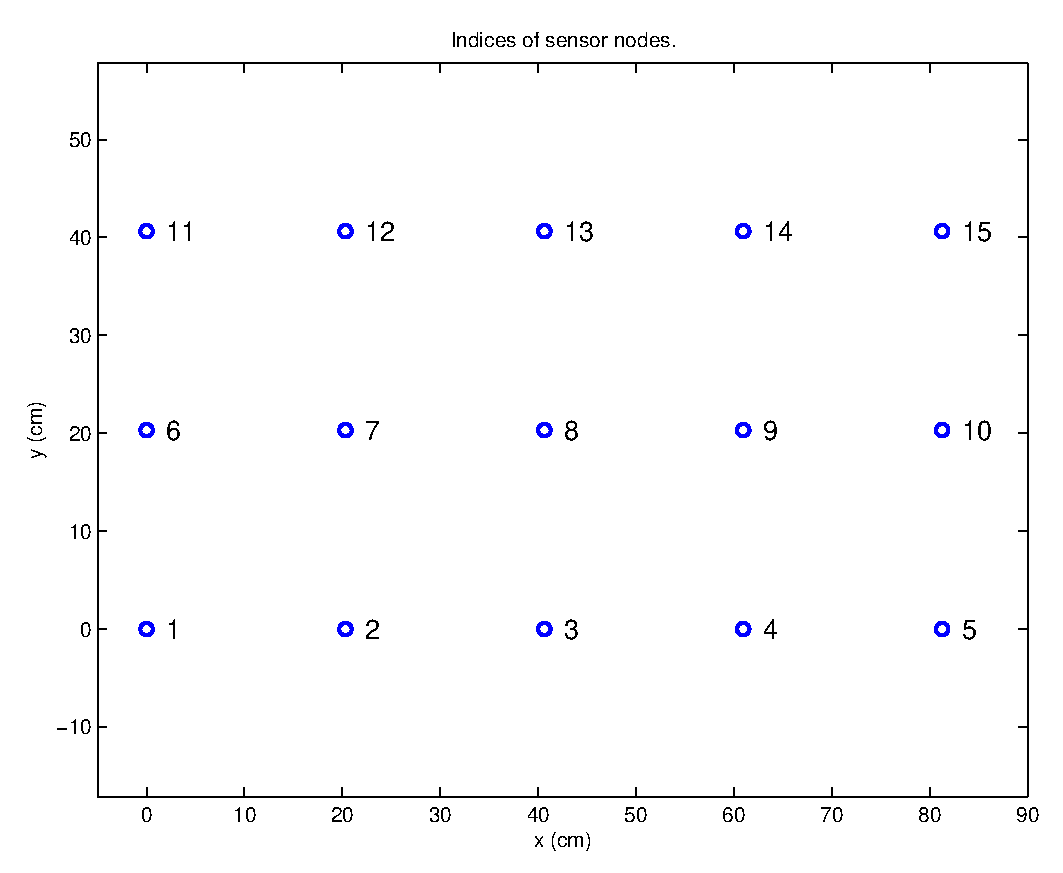
\includegraphics[width=0.8\textwidth]{img/IndexSenNode}
\caption{The indices for sensor nodes of the sensor selection testbed.}\label{f:indSenNode}
\end{figure}
\afterpage{\clearpage}


\begin{itemize}
\item The variable \verb!est! is the estimate on the position of the lamp. The indices of \verb!est! are associated with the testing points with the same indices. The indices of the testing points are shown in Fig.~\ref{f:indices}. The first row of \verb!est!\{i,j\} are the manually measured positions in inches. From left to right, the three entries in the row are the $x$, $y$ positions and the estimated positioning error, respectively. Since the estimated positioning errors for the manual measurement are invalid, it is always 0 for each \verb!est!\{i,j\} matrix.
\item The second row of each \verb!est!\{i,j\} matrices is the a priori estimates on the lamp's position, with the three entries still $x$, $y$ and positioning error respectively, from left to right. The values are still measured by inches.
\item From the forth to the last rows of the \verb!est!\{i,j\} matrices are the a posterior estimates whose formate follows the same convention of the a priori estimate in the second row.
\item The matrix \verb!SamplingRate! are the sampling rates after the sensor selection.
    The rows of the matrix \verb!SamplingRate!, from the first to the last one, are the outputs for position (1,1), (1,2), $\cdots$, (1,7), (2,1), $\cdots$, (3,7), respectively. The indices are commented on the right of each row.
    The columns of the matrix \verb!SamplingRate! are the sampling rates for each sensor nodes, ordered by the indices of the sensor nodes. The indices are shown in Fig.~\ref{f:indSenNode}.
        The total sample number is 255. Due to the rounding errors, the summation of each row may not be 255 exactly.
\item The matrix \verb!LampData! is the experimental data used to plot Figs.~\ref{f:sensorIID}, \ref{f:SensorFit} and \ref{f:corcoef}. The data characterize halogen lamps as well as the Tmote Sky sensor nodes.
     The columns of the matrix are the data sets collected at distances from 0 cm to 50.8 cm, with 50.8 cm apart. The rows of the matrix are ordered by the 100 trials.
\end{itemize}



%\clearpage
\renewcommand{\baselinestretch}{0.5}
\twocolumn
\tiny
%% \scriptsize % too big font
%\begin{lstlisting}
\begin{verbatim}
est=cell{3,7};
est{1,1}=[
    3.8, 3, 0
    4.0474831836304,3.98640937729381,0.530539616068237
    3.69030219368631,4.53084046791177,0.245608597232329
    3.79360998078517,4.44047335771038,0.247284311837911
    3.79621500159606,4.43812979567396,0.247333701041882
    3.79900725974776,4.43551236073322,0.247378113526514
    3.80174302218333,4.43300988735921,0.247426551668037
    3.80420788178024,4.43078235024581,0.247473424908412
    3.80711507842732,4.42857523620138,0.2475153769021
    3.8097045499778,4.42617335224803,0.247561259612977
    3.81176453716081,4.42382284651583,0.24760574512124
    3.81405626047611,4.42173848606945,0.247644785685762
];

est{1,2}=[
    7.6, 3.3, 0
    8.04844648870563,4.10461796931969,0.474034178884049
    7.78988705044351,3.26877842057838,0.218798813393424
    7.85778583557264,3.70231012279228,0.221532654441194
    7.86192679005886,3.72254326525508,0.221677350012992
    7.86268122779319,3.72599101036754,0.221704707275966
    7.86299442102457,3.72896057293481,0.221729475943818
    7.86372897760968,3.7322146762133,0.221751784546935
    7.86424004209608,3.73548455575158,0.221775182307836
    7.86498119492832,3.73878126829728,0.221799368202466
    7.86546919166884,3.741852517379,0.221823167916907
    7.86618793195867,3.74495644064239,0.221845942306571
];

est{1,3}=[
    12, 2.8, 0
    12.5301623430214,3.4021758557392,0.528036383294451
    12.5294420397135,3.40524153336293,0.242459389292195
    12.7900441996901,3.0685666537424,0.244938500366456
    12.7928760010253,3.06620515984053,0.24495991350521
    12.8010155606284,3.04736388574673,0.245080711854237
    12.8038350664367,3.04584990716162,0.245104828795585
    12.8061397485558,3.04342702829233,0.245116957274766
    12.8078170282549,3.04069913993192,0.245134405943397
    12.8107497109872,3.03951915959153,0.245153243198329
    12.8129271275762,3.03667948673614,0.24516325582619
    12.8152575286711,3.0351250374991,0.245183184291676
];

est{1,4}=[
    15.3, 3.1, 0
    15.8323772861596,3.65729018727796,0.476469782144612
    15.7879022162631,4.68445564682164,0.226131498088571
    15.6094905438954,4.34808463598548,0.226633922743073
    15.5944614710543,4.32868423969731,0.226655668424468
    15.5922960059422,4.32588507176634,0.226658829730532
    15.5899486989545,4.32304366225173,0.226662274784185
    15.587849219258,4.32040412899407,0.22666504665521
    15.5853176349295,4.31757584665639,0.226668107160708
    15.5830726106713,4.31496905726211,0.226669969841257
    15.581110799512,4.31218027172983,0.226672212266429
    15.5791772636353,4.30947082400796,0.226676968931825
];

est{1,5}=[
    19.2, 3.2, 0
    20.2149398942565,3.92034236110996,0.497836240088391
    19.8041844512562,4.44360025388118,0.247456076130034
    19.8137229503216,4.42591174170551,0.247599608866044
    19.8352920332063,4.40095468039268,0.24800671934566
    19.8380717408332,4.3983204475248,0.248054573553278
    19.84124132214,4.39623280729016,0.248102097784305
    19.8441247815937,4.3939165385831,0.248148654855953
    19.8464684242864,4.39164588066321,0.248194386207589
    19.8475911944007,4.38871336871884,0.248234695550386
    19.8496789947044,4.38630470486163,0.248269122587239
    19.8514765997059,4.38371663964075,0.248308105433175
];

est{1,6}=[
    23,3.3, 0
    23.4269705135168,4.12908722018588,0.474318308701361
    24.1851374508688,3.47794833112922,0.262776502012932
    24.2056483211575,3.9096396046454,0.262622132598746
    24.2264813432486,3.94906325937053,0.263038148207259
    24.2366940949596,3.96696274390946,0.263267420558916
    24.2384594543067,3.96973520112174,0.263312607391327
    24.2399539702703,3.97230541432262,0.263353172150807
    24.2401667566297,3.97419000623648,0.263387378212243
    24.2397707185921,3.9753254663463,0.26339083429375
    24.2389034355644,3.97659349865715,0.26338005871795
    24.2382601756784,3.97792301541945,0.263357603249006
];

est{1,7}=[
    26.8, 3.6, 0
    27.5725386207448,4.80468523153953,0.526022594967061
    27.5733024278611,4.66731049947225,0.245229750431927
    27.5738603104731,4.66361680980554,0.24517038515931
    27.4633925778482,5.07147056596402,0.25262593132801
    27.4618030342764,5.07487018164453,0.252701019037374
    27.4601343301208,5.07826269715765,0.25277433985669
    27.4583153821469,5.08130138199575,0.252847446347764
    27.4568222667089,5.0840248556857,0.252912088257293
    27.4553609680044,5.08668047409301,0.252970565270152
    27.4778290153921,5.14803823223532,0.258296660822031
    27.4759928106581,5.15566491531472,0.25853433991981
];

est{2,1}=[
    3.8, 7.6, 0
    5.19247472077239,8.38626785551865,0.49245825836639
    5.43855852814086,6.49575163166598,0.238726884130604
    5.5300084799918,7.10290308856285,0.24328769866985
    5.52910155290043,7.10647917238645,0.243327004516333
    5.52867208536207,7.1103902502845,0.243364510889071
    5.52815725289167,7.11405857387911,0.243402383757097
    5.52716529095717,7.11732101151381,0.243438544988974
    5.52659728528346,7.12070011516655,0.243473726119788
    5.52561928174833,7.12390084768421,0.243507584298037
    5.52431571702406,7.12715308779106,0.243542151471669
    5.52338333241307,7.1303280332901,0.243579043105776
];

est{2,2}=[
    7, 6.9, 0
    7.10351390415587,8.32211001953104,0.464904533379217
    7.09131262087992,7.2554386028169,0.23626064828166
    7.04588829045246,7.71837183698774,0.239454026071859
    7.04518147964838,7.72218286752515,0.239476836274018
    7.04446875842448,7.72594293632048,0.239497629139189
    7.0433738340172,7.7419728070872,0.239575090596243
    7.04253675693438,7.74545167873637,0.239593382648254
    7.04124341296261,7.7487642276587,0.239611972979637
    7.04031124217408,7.75228932892047,0.239631773136892
    7.03906564388669,7.75552739139764,0.239650603090459
    7.03768523759128,7.75860358114261,0.23966950681079
];

est{2,3}=[
    11.2, 7.3, 0
    12.7244546498609,7.91581685936649,0.474274559157398
    12.5944366152738,7.85704092796102,0.231102058331098
    12.591537434999,7.85563722171299,0.23106004344745
    12.5886320314792,7.85404592076225,0.231025323588074
    12.585908215043,7.85271958407035,0.23098980925528
    12.5827664259719,7.85118631665943,0.230957258695373
    12.5797194670246,7.84969279228447,0.230919757107458
    12.5772644430512,7.84847946835278,0.230883419758822
    12.5749837136277,7.84706766596286,0.23085414324467
    12.5726716650092,7.845922008459,0.230825809168539
    12.5708351814446,7.84482436471876,0.230798297213902
];

est{2,4}=[
    15.5, 7.8, 0
    14.4356781955664,9.13675562635047,0.470559229881083
    14.1454778673083,9.01483418485509,0.248127537728326
    14.143358809858,9.01154854031136,0.248074608122404
    14.368104182344,8.95601449695197,0.249753138574824
    14.3718628056138,8.95582478389369,0.249794249846502
    14.3749876242079,8.95559282408547,0.24983990686404
    14.3780523281553,8.95513520343895,0.249877065358886
    14.3808979800278,8.95500626963005,0.249910451350276
    14.3840088741955,8.95469284110166,0.249945833614049
    14.386980268267,8.9544311250481,0.249982260932188
    14.3898950030945,8.95454994472526,0.250017790346692
];

est{2,5}=[
    19.5, 7.5, 0
    20.8715408008781,7.88007813823719,0.480274061779725
    19.7766467180037,7.90031835501856,0.230224568977455
    19.7740648486673,7.90056936338291,0.230205511946842
    20.2711164479792,7.59689858755187,0.23118118443546
    20.2740859061849,7.59465458271047,0.231188390585385
    20.2764833105639,7.59219954845736,0.231197205167541
    20.2780255479161,7.58970730319232,0.231200907008055
    20.2795269056123,7.58726615144305,0.231198415148742
    20.2814949114178,7.5846904969913,0.231195982858905
    20.2836921022796,7.58243955755335,0.231196234462091
    20.2859220869828,7.58044548217516,0.231199936578724
];

est{2,6}=[
    23.5, 7, 0
    23.2291287259428,8.52600994778599,0.464769169249906
    24.1919734328888,6.19244286700353,0.234933041834163
    24.2185858725472,6.49483621453919,0.234684813943579
    24.2202262258969,6.49799063581697,0.234688540982829
    24.2218764542288,6.50078961639374,0.234694268612303
    24.2232078501157,6.50397743826536,0.234700348734883
    24.2247957811767,6.50720445733702,0.234704580980775
    24.2261369592064,6.51034059285691,0.234710095874418
    24.2274975456499,6.51289674726909,0.234714484578506
    24.2295032681051,6.51455788136657,0.234719417957237
    24.2314938776745,6.51638141608923,0.234728222249876
];

est{2,7}=[
    27.3, 8, 0
    28.5928281003494,8.51380349863577,0.46953183590475
    28.7191276728031,7.26318106148668,0.219098408199878
    28.2782765639044,7.64465664621348,0.220281684340674
    28.2761619143566,7.64781956109518,0.220293441637172
    28.2745972443569,7.65069776320583,0.220304983306441
    28.2726018200144,7.65376146955409,0.220314151541114
    28.2706706587754,7.65677468057445,0.220325323920195
    28.2688017692495,7.65973831911525,0.220336289276854
    28.2669932189114,7.66265328743853,0.220347050895101
    28.2648637221324,7.66555046382949,0.220357612057879
    28.2632847975459,7.66816781891551,0.22036953845711
];

est{3,1}=[
    3.5, 11.7, 0
    3.09687762311607,12.5689839394288,0.555780502598974
    3.92359954309961,12.1001918512246,0.238470752046229
    3.94391559619304,12.0982973141513,0.238324441753265
    3.98799444479162,12.1067602577344,0.238054228823887
    4.02573235673257,12.120021143127,0.237853616152455
    4.06264798146971,12.1379265487523,0.237685400797833
    4.10684749231686,12.1647741912006,0.237518396400454
    4.1360872669641,12.1845313243231,0.237425067643203
    4.20268688562826,12.2259465660745,0.237231572809417
    4.417049431429,12.3516375693853,0.236817116445147
    4.41595406306127,12.3503609142533,0.236811748000578
];

est{3,2}=[
    8, 11.2, 0
    8.48182696704214,12.3442172791527,0.494885545009503
    8.39393545173675,12.3407335754648,0.263934849712607
    8.39008436610658,12.3407959058925,0.263912542174231
    8.37423391186283,12.340764581803,0.263822614654134
    8.37042123269111,12.3411751518556,0.263799878451527
    8.36677627616588,12.3413320744812,0.263772673445137
    8.3631984259023,12.3426464193286,0.263749387885431
    8.35969718737714,12.3435065379197,0.263712345331416
    8.35627277542459,12.3439369450584,0.263681158070238
    8.35262690955769,12.3438715710763,0.26365551464843
    8.34928357483886,12.3443114512877,0.263634400596631
];

est{3,3}=[
    12.1, 10.8, 0
    12.1545258924819,12.14087220982,0.51969478800259
    12.4587856607152,11.9086271237921,0.241023229865354
    13.086612409275,12.099189461058,0.250191524091398
    13.0164085332725,12.3474567130655,0.248734125918859
    13.0628151138377,12.3248090794699,0.24946032031902
    12.9751933397787,12.5444239460777,0.247800249333395
    13.2274154863334,12.3665948980713,0.252343481984132
    13.188742043957,12.5074728986228,0.251341392946569
    13.1565165908766,12.5726132698614,0.250615013478188
    13.155106399523,12.5746932480242,0.250576550664049
    13.1561131076997,12.5748755752769,0.250546945157326
];

est{3,4}=[
    15.2, 11.6, 0
    14.5526142604682,12.2590462449459,0.482024832778939
    13.9351282158724,12.2989834503444,0.284945766294924
    14.142758115211,12.2412202647842,0.298551486143719
    14.146009875663,12.2403092631596,0.298838121625628
    14.149216411208,12.2394253841412,0.299083219504926
    14.1520822111325,12.2392461100974,0.299325613820961
    14.1549064064729,12.2390644044544,0.299540326352619
    14.1578374380442,12.2385410682676,0.299752537720442
    14.1607271037254,12.2380296811226,0.2999748162573
    14.1636071971757,12.2379378730859,0.30019456715541
    14.1665927789055,12.237500079389,0.300412446316843
];

est{3,5}=[
    19.6, 11.2, 0
    20.1759974569403,11.8348526478546,0.525240604622037
    20.2625320853757,11.8436422478968,0.239340098732339
    20.2663230715709,11.8435260899923,0.2393690472123
    20.270001607495,11.8433639373404,0.239397353851925
    20.2738216285464,11.8433836763175,0.239425031959896
    20.0582650101058,12.0042005207837,0.25282291302391
    20.0593964397805,12.0028386822792,0.252843778237171
    20.0605120159667,12.0015030904996,0.252860489901919
    20.0616118527779,12.0001931721269,0.252876896153131
    20.0629365807236,11.9991452437586,0.25289300271723
    20.0639969143623,11.9978689664111,0.252908925627841
];

est{3,6}=[
    23.8, 11.5, 0
    25.4209886143985,12.2126252022009,0.500049229713879
    25.4333491965396,12.0772573192592,0.2474726875701
    25.4602379287259,12.2715976242901,0.24656359758152
    25.4609098737801,12.275270820689,0.24654718352942
    25.4613058889895,12.2786174745469,0.246530483425011
    25.4616768785831,12.2817953217742,0.246516357548666
    25.4619037089963,12.284459772763,0.246503020026926
    25.4620899920182,12.2877058887874,0.246492272070595
    25.4622770874241,12.2900742340604,0.246479644524678
    25.4625684007942,12.292676863969,0.246470221876805
    25.4626979111883,12.2955108497618,0.246459498137656
];

est{3,7}=[
    26.4, 11.5, 0
    27.3900942961187,11.601454487046,0.52302180705273
    27.3883920167765,11.6024585113237,0.244532340543695
    26.8275215897316,11.4284901254502,0.254476312425801
    26.8180378780527,11.4209831453314,0.254681941268781
    26.8071181328237,11.4159366048291,0.254906896641411
    26.8041412341345,11.4149053971816,0.254984741434298
    26.8009465493263,11.4130126194084,0.255051584540131
    26.7981575167954,11.4115767621728,0.255120500091348
    26.7957080954625,11.4099972140854,0.255181611407412
    26.793318451826,11.4084582394704,0.255234152693239
    26.7909871520897,11.4069588622595,0.255285495600224
];


SamplingRate=[
 84, 84, 0, 0, 0, 0, 84, 0, 0, 0, 0, 0, 0, 0, 0 %1,1
 0, 0, 0, 0, 0, 59, 117, 77, 0, 0, 0, 0, 0, 0, 0 %1,2
 0, 74, 125, 0, 0, 0, 0, 55, 0, 0, 0, 0, 0, 0, 0 %1,3
 0, 100, 121, 33, 0, 0, 0, 0, 0, 0, 0, 0, 0, 0, 0 %1,4
 0, 0, 84, 84, 0, 0, 0, 0, 84, 0, 0, 0, 0, 0, 0 %1,5
 0, 0, 2, 0, 0, 0, 0, 125, 126, 0, 0, 0, 0, 0, 0 %1,6
 0, 0, 0, 19, 0, 0, 0, 0, 126, 109, 0, 0, 0, 0, 0 %1,7
 0, 0, 0, 0, 0, 84, 84, 0, 0, 0, 0, 84, 0, 0, 0 %2,1
 0, 0, 0, 0, 0, 84, 84, 0, 0, 0, 0, 84, 0, 0, 0 %2,2
 0, 0, 88, 0, 0, 0, 0, 121, 0, 0, 0, 0, 45, 0, 0 %2,3
 0, 0, 0, 0, 0, 0, 32, 114, 0, 0, 0, 0, 108, 0, 0 %2,4
 0, 0, 0, 100, 0, 0, 0, 0, 123, 0, 0, 0, 0, 31, 0 %2,5
 0, 0, 0, 0, 0, 0, 0, 84, 84, 0, 0, 0, 0, 84, 0 %2,6
 0, 0, 0, 0, 0, 0, 0, 0, 112, 0, 0, 0, 0, 67, 74 %2,7
 0, 0, 0, 0, 0, 88, 0, 0, 0, 0, 124, 41, 0, 0, 0 %3,1
 0, 0, 0, 0, 0, 0, 84, 0, 0, 0, 0, 84, 84, 0, 0 %3,2
 0, 0, 0, 0, 0, 0, 0, 93, 0, 0, 0, 34, 127, 0, 0 %3,3
 0, 0, 0, 0, 0, 0, 0, 123, 0, 0, 0, 0, 120, 11, 0 %3,4
 0, 0, 0, 0, 0, 0, 0, 44, 127, 0, 0, 0, 0, 83, 0 %3,5
 0, 0, 0, 0, 0, 0, 0, 0, 33, 0, 0, 0, 0, 116, 105 %3,6
 0, 0, 0, 0, 0, 0, 0, 0, 126, 22, 0, 0, 0, 105, 0 %3,7
];

LampData=[...
6799, 5773, 4901, 3900, 3356, 2758, 2459, 2423, 2032, 2160, 2178;...
6750, 5639, 4797, 3967, 3350, 2783, 2459, 2416, 2056, 2166, 2185;...
6738, 5780, 4919, 3918, 3363, 2795, 2478, 2416, 2026, 2148, 2197;...
6787, 5749, 4852, 3887, 3381, 2777, 2441, 2429, 2020, 2142, 2215;...
6805, 5639, 4772, 3918, 3405, 2770, 2447, 2429, 2026, 2166, 2178;...
6768, 5798, 4852, 3979, 3375, 2819, 2484, 2404, 2020, 2166, 2191;...
6750, 5755, 4931, 3967, 3344, 2764, 2484, 2404, 2032, 2166, 2191;...
6787, 5651, 4797, 3900, 3332, 2795, 2465, 2404, 2038, 2142, 2172;...
6744, 5682, 4797, 3881, 3356, 2801, 2465, 2435, 2020, 2142, 2178;...
6726, 5798, 4901, 3912, 3399, 2777, 2459, 2410, 2038, 2166, 2203;...
6750, 5670, 4772, 3967, 3344, 2783, 2484, 2410, 2020, 2166, 2191;...
6781, 5651, 4840, 3955, 3363, 2789, 2459, 2416, 2020, 2142, 2191;...
6762, 5755, 4925, 3869, 3369, 2764, 2478, 2429, 2038, 2136, 2209;...
6726, 5798, 4846, 3881, 3417, 2789, 2465, 2410, 2050, 2172, 2209;...
6726, 5712, 4766, 3918, 3399, 2795, 2459, 2410, 2026, 2160, 2203;...
6750, 5682, 4888, 3973, 3375, 2770, 2453, 2423, 2020, 2172, 2209;...
6707, 5767, 4791, 3942, 3350, 2801, 2496, 2410, 2050, 2154, 2209;...
6732, 5780, 4797, 3894, 3363, 2801, 2478, 2435, 2056, 2178, 2197;...
6756, 5694, 4925, 3875, 3405, 2777, 2447, 2410, 2044, 2142, 2185;...
6774, 5633, 4888, 3948, 3399, 2783, 2453, 2416, 2026, 2154, 2203;...
6707, 5712, 4785, 3967, 3369, 2770, 2465, 2423, 2044, 2154, 2191;...
6732, 5798, 4919, 3918, 3356, 2801, 2465, 2423, 2056, 2160, 2185;...
6781, 5780, 4779, 3857, 3369, 2764, 2484, 2423, 2062, 2172, 2197;...
6774, 5676, 4815, 3875, 3411, 2770, 2471, 2423, 2044, 2148, 2178;...
6726, 5651, 4901, 3936, 3405, 2795, 2453, 2398, 2050, 2172, 2197;...
6738, 5706, 4797, 3955, 3363, 2770, 2465, 2423, 2032, 2166, 2215;...
6756, 5737, 4797, 3912, 3363, 2783, 2459, 2404, 2026, 2160, 2197;...
6719, 5639, 4882, 3851, 3405, 2770, 2465, 2435, 2026, 2166, 2203;...
6713, 5633, 4919, 3875, 3417, 2770, 2465, 2429, 2044, 2142, 2209;...
6774, 5731, 4821, 3900, 3393, 2807, 2453, 2392, 2056, 2142, 2209;...
6719, 5786, 4840, 3948, 3363, 2795, 2447, 2416, 2044, 2160, 2197;...
6707, 5609, 4754, 3887, 3405, 2801, 2496, 2410, 2026, 2148, 2215;...
6750, 5682, 4833, 3869, 3387, 2758, 2484, 2404, 2062, 2160, 2191;...
6774, 5786, 4846, 3918, 3363, 2777, 2478, 2404, 2056, 2148, 2197;...
6726, 5761, 4803, 3961, 3375, 2807, 2484, 2386, 2044, 2172, 2209;...
6701, 5645, 4919, 3948, 3411, 2770, 2484, 2423, 2056, 2166, 2197;...
6719, 5633, 4901, 3900, 3387, 2783, 2465, 2429, 2032, 2172, 2203;...
6756, 5798, 4876, 3875, 3332, 2770, 2453, 2423, 2056, 2148, 2185;...
6744, 5633, 4925, 3912, 3399, 2770, 2465, 2404, 2038, 2185, 2191;...
6689, 5700, 4809, 3961, 3405, 2770, 2459, 2416, 2038, 2154, 2215;...
6707, 5810, 4760, 3924, 3356, 2764, 2465, 2398, 2044, 2172, 2215;...
6756, 5731, 4827, 3869, 3363, 2795, 2441, 2404, 2050, 2148, 2185;...
6750, 5798, 4919, 3851, 3405, 2795, 2447, 2416, 2026, 2178, 2209;...
6707, 5737, 4888, 3900, 3430, 2795, 2478, 2404, 2050, 2166, 2209;...
6701, 5633, 4785, 3924, 3375, 2795, 2459, 2386, 2044, 2154, 2191;...
6750, 5682, 4785, 3948, 3363, 2770, 2471, 2429, 2056, 2148, 2191;...
6713, 5780, 4913, 3930, 3411, 2789, 2441, 2410, 2062, 2166, 2185;...
6695, 5633, 4901, 3881, 3399, 2801, 2478, 2404, 2056, 2178, 2215;...
6726, 5670, 4791, 3863, 3338, 2764, 2478, 2410, 2038, 2160, 2209;...
6726, 5773, 4913, 3869, 3375, 2807, 2490, 2416, 2044, 2166, 2215;...
6695, 5657, 4901, 3894, 3411, 2795, 2441, 2410, 2050, 2166, 2221;...
6707, 5633, 4797, 3930, 3399, 2758, 2484, 2410, 2038, 2154, 2185;...
6750, 5725, 4803, 3961, 3363, 2783, 2484, 2410, 2050, 2172, 2209;...
6726, 5773, 4925, 3900, 3350, 2777, 2465, 2398, 2050, 2154, 2209;...
6713, 5725, 4901, 3863, 3417, 2777, 2478, 2398, 2032, 2160, 2203;...
6756, 5639, 4797, 3887, 3405, 2770, 2453, 2435, 2038, 2160, 2215;...
6707, 5725, 4901, 3930, 3338, 2801, 2478, 2398, 2062, 2160, 2191;...
6683, 5786, 4797, 3948, 3399, 2770, 2471, 2398, 2038, 2166, 2209;...
6726, 5700, 4772, 3912, 3405, 2807, 2471, 2386, 2032, 2185, 2197;...
6744, 5590, 4901, 3845, 3356, 2801, 2465, 2429, 2050, 2172, 2191;...
6701, 5615, 4901, 3881, 3363, 2795, 2459, 2392, 2056, 2166, 2215;...
6726, 5700, 4791, 3900, 3393, 2758, 2484, 2404, 2038, 2178, 2191;...
6750, 5761, 4882, 3955, 3350, 2789, 2459, 2398, 2044, 2172, 2209;...
6689, 5731, 4895, 3948, 3387, 2770, 2459, 2410, 2044, 2166, 2209;...
6689, 5633, 4797, 3875, 3417, 2807, 2471, 2404, 2062, 2178, 2209;...
6732, 5657, 4785, 3839, 3381, 2795, 2459, 2404, 2069, 2185, 2221;...
6701, 5761, 4901, 3851, 3393, 2832, 2465, 2404, 2038, 2166, 2221;...
6689, 5786, 4760, 3936, 3424, 2801, 2478, 2410, 2056, 2178, 2197;...
6726, 5688, 4772, 3900, 3393, 2801, 2465, 2386, 2062, 2185, 2203;...
6713, 5609, 4870, 3851, 3350, 2777, 2496, 2410, 2038, 2185, 2203;...
6677, 5633, 4901, 3863, 3363, 2777, 2484, 2404, 2032, 2166, 2215;...
6701, 5712, 4766, 3894, 3411, 2819, 2465, 2423, 2056, 2160, 2227;...
6738, 5792, 4901, 3924, 3350, 2825, 2453, 2386, 2050, 2185, 2203;...
6738, 5731, 4809, 3863, 3356, 2770, 2459, 2410, 2056, 2166, 2191;...
6701, 5651, 4772, 3851, 3381, 2801, 2478, 2392, 2044, 2154, 2209;...
6671, 5621, 4913, 3900, 3430, 2795, 2453, 2410, 2056, 2178, 2215;...
6719, 5706, 4797, 3948, 3387, 2783, 2453, 2429, 2062, 2185, 2215;...
6744, 5633, 4913, 3875, 3363, 2777, 2471, 2416, 2038, 2191, 2203;...
6707, 5645, 4870, 3900, 3350, 2807, 2459, 2392, 2032, 2166, 2203;...
6671, 5657, 4779, 3948, 3411, 2770, 2441, 2429, 2056, 2160, 2221;...
6707, 5633, 4827, 3948, 3369, 2770, 2447, 2410, 2056, 2166, 2197;...
6738, 5676, 4919, 3863, 3332, 2783, 2465, 2410, 2044, 2178, 2227;...
6701, 5798, 4809, 3948, 3375, 2783, 2484, 2404, 2038, 2166, 2227;...
6665, 5627, 4791, 3942, 3399, 2764, 2478, 2392, 2038, 2172, 2209;...
6707, 5621, 4888, 3875, 3411, 2764, 2465, 2410, 2044, 2160, 2227;...
6744, 5712, 4766, 3845, 3369, 2819, 2490, 2404, 2038, 2166, 2227;...
6707, 5761, 4840, 3918, 3375, 2813, 2459, 2410, 2044, 2185, 2221;...
6677, 5609, 4919, 3967, 3405, 2795, 2459, 2410, 2069, 2191, 2221;...
6726, 5657, 4821, 3936, 3356, 2807, 2484, 2392, 2069, 2178, 2209;...
6744, 5731, 4779, 3845, 3399, 2813, 2453, 2404, 2032, 2172, 2215;...
6683, 5798, 4876, 3851, 3405, 2783, 2465, 2429, 2069, 2160, 2197;...
6683, 5755, 4913, 3918, 3405, 2777, 2471, 2404, 2038, 2185, 2233;...
6738, 5670, 4803, 3948, 3338, 2795, 2459, 2410, 2038, 2191, 2209;...
6677, 5609, 4913, 3851, 3375, 2807, 2459, 2404, 2056, 2197, 2221;...
6701, 5645, 4779, 3900, 3430, 2813, 2471, 2410, 2069, 2166, 2197;...
6732, 5725, 4840, 3967, 3381, 2795, 2465, 2416, 2056, 2178, 2233;...
6677, 5767, 4943, 3912, 3356, 2777, 2471, 2410, 2044, 2172, 2215;...
6695, 5700, 4864, 3845, 3381, 2783, 2471, 2404, 2075, 2191, 2233;...
6744, 5621, 4772, 3887, 3411, 2801, 2465, 2392, 2044, 2185, 2233;...
6726, 5627, 4858, 3942, 3399, 2801, 2478, 2410, 2050, 2185, 2227];
\end{verbatim}
%\end{lstlisting}
%%\renewcommand{\baselinestretch}{1}


%\section{Beacon Placement}

%\section{MAS-net Platform}
%\section{Target Tracking on MAS-net Platform}
